


% Não é necessário alterar nada nesta primeira parte, esta primeira parte consiste na parte de configuração da linguagem e da formatação mais bruta do boletim epidemiológico %





%%%%%%%%%%%%%%%%%%%%%%%%%%%%%%%%%%%%%%%%%%%%%%%%%%%%%%%%%%%%%%%%%%%%%%%%%
% Este é um documento que servirá de modelo para                        
% os Boletins Epidemiológicos produzidos pela Sala de Situação de Saúde 
% da Faculdade de Saúde - UnB                                           
%%%%%%%%%%%%%%%%%%%%%%%%%%%%%%%%%%%%%%%%%%%%%%%%%%%%%%%%%%%%%%%%%%%%%%%%%








% INÍCIO DA PRIMEIRA PARTE - NÃO ALTERAR NADA %


\documentclass{article}
\usepackage{scrextend} %pacote pra ajustar tamanho da fonte
\usepackage{moresize} %pacote pra mais opções tamanho da fonte (permite HUGE e ssmall)
\usepackage[utf8]{inputenc}
\usepackage{graphicx,wrapfig}
\usepackage{eso-pic}
\usepackage{ifthen}
\usepackage{lipsum}
\usepackage{graphicx}
\usepackage{xcolor}
\usepackage{multicol} %pacote pra usar colunas de texto
\setlength{\columnsep}{1.5cm}
\usepackage[a4paper, total={7in, 8in}]{geometry}
\usepackage[explicit]{titlesec}
\usepackage[absolute,overlay]{textpos}
\usepackage{indentfirst} %pacote que deixa inicio paragrafo identado
\usepackage[hidelinks]{hyperref} %pacote pra referencias
\usepackage{url}
\hypersetup{ %%configura aparencia link da referencia
   colorlinks,
   %linkcolor={red!50!black},
   %citecolor={blue!50!black},
   urlcolor={blue!80!black}
}

\usepackage{ragged2e} %Para usar o comando que justifica o texto
\usepackage{fontspec}
\setmainfont[BoldItalicFont=Myriad_Bold_Italic.ttf, BoldFont=MyriadPro-Bold.otf, ItalicFont=MyriadPro-It.otf]{MyriadPro-Regular.otf} %% Config. para usar fonte Myriad Pro cujo arquivos estão na pasta do projeto

\newfontfamily{\titlefont}[BoldItalicFont=CambriaBoldItalic.ttf, BoldFont=CambriaBold.ttf, ItalicFont=CambriaItalic.ttf]{Cambria.ttf}  %%Config para usar fonte Cambria cujo arquivos estão na pasta do projeto

\newfontfamily{\calibrifont}[BoldItalicFont=CalibriBoldItalic.ttf, BoldFont=CalibriBold.ttf, ItalicFont=CalibriItalic.ttf]{Calibri.ttf}%%Config para usar fonte Calibri cujo arquivos estão na pasta do projeto
\DeclareTextFontCommand{\calibri}{\calibrifont}%% permite usar calibri da forma: \calibri{texto em calibri}

\newfontfamily{\timesfont}[BoldItalicFont=times-new-roman-bold-italic.ttf, BoldFont=times-new-roman-bold.ttf, ItalicFont=times-new-roman-italic.ttf]{TimesNewRoman.ttf} %%Config. para usar fonte Times New Roman cujo arquivos estão na pasta do projeto






% FIM DA PRIMEIRA PARTE - NÃO ALTERAR NADA DA PRIMEIRA PARTE%







% INÍCIO DA PÁGINA 2




\title{
\textbf{\HUGE{\titlefont Boletim Epidemiológico}} % Nesta linha é colocado o título maior do boletim, para ser alterado é necessário apenas trocar o nome dentro da chaves, por exemplo: trocar Boletim Epidemiológico para Boletim da Saúde
\\
\small{\calibrifont Análise Epidemiológica dos casos de Febre Amarela. Até a semana} % Nesta linha é colocado o subtítulo que fica abaixo do título principal da página, para alterar é necessário trocar a frase dentro da chaves na cor preta pela frase desejada
\\
\small{\calibrifont Epidemiológica 18 de 2018.} % Nesta linha é colocado a continuação da frase de subtítulo, ela é colocada separada por questão de estética de formatação da página, ou seja, esta linha fica exatamente abaixo do subtítulo e contem a data, para alteração é necessário trocar a frase dentro da chaves na cor preta pela frase desejada
}





\date{} % NÃO ALTERAR ESTA LINHA- retira a numeração das paginas - NÃO ALTERAR ESTA LINHA%
\pagenumbering{gobble}






\begin{document}

%capa do boletim%
\AddToShipoutPictureBG{\ifthenelse{\value{page}>1}{}{
\includegraphics[width=\paperwidth,height=\paperheight]{capa_boletim_epidemiologico.png}}} % Este espaço serve para colocar a imagem da capa inicial da primeira página, a imagem irá aparecer justificado em harmonia com o texto colocado, para alterar a imagem basta inserir a imagem no canto superior esquerdo na aba "project", e assim irá abrir uma nova aba escrito "file", agora é necessário clicar na palavra "files" que está na cor cinza com um ícone de pasta ao lado, quando clicado no ícone "file" irá abrir uma janela com várias opções, aí é necessário selecionar a 9ª opção denominada "computer" que está no subitem uploade... computer, a escolha é de selecionar a imagem do computador e após a escolha é necessário clicar em enviar; após fazer isso é necessário observar qual o nome da imagem, e aí é necessário apenas acrescentar o nome da imagem nas chaves abaixo, conforme exemplo {capa_boletim_epidemiologico.png} é necessário colocar a extensão da imagem (no caso o .png), caso a imagem seja .jpg é necessário alterar o .png para o .jpg %
\begin{frame}{}
\end{frame} 



\AddToShipoutPictureBG{\ifthenelse{\value{page}>1}{
 \put(0,785){{
\includegraphics[width=\paperwidth]  {img_cabecalho_boletim_epidemiologico.png}}}}
} % Este espaço serve para colocar a imagem de cabeçalho da capa inicial da primeira página, a imagem irá aparecer justificado em harmonia com o texto colocado, para alterar a imagem basta inserir a imagem no  canto superior esquerdo na aba "project", e assim irá abrir uma nova aba escrito "file", agora é necessário clicar na palavra "files" que está na cor cinza com um ícone de pasta ao lado, quando clicado no ícone "file" irá abrir uma janela com várias opções, aí é necessário selecionar a 9ª opção denominada "computer" que está no subitem uploade... computer, a escolha é de selecionar a imagem do computador e após a escolha é necessário clicar em enviar;; após fazer isso é necessário observar qual o nome da imagem, e aí é necessário apenas acrescentar o nome da imagem nas chaves abaixo, conforme exemplo {img_cabecalho_boletim_epidemiologico.png} é necessário colocar a extensão da imagem (no caso o .png), caso a imagem seja .jpg é necessário alterar o .png para o .jpg %





\newpage % nova pagina %



% título do documento(Boletim Epidemiologico)%

\vspace*{-85pt}
    {\let\newpage\relax\maketitle}
\begin{textblock*}{10cm}(15.5cm,3.5cm) % {largura do bloco} (coordenadas) 

   \small{Volume 1} % Esta linha é utilizada para colocar qual o volume do boletim epidemiológico, neste caso o volume 1%  
   
     \small{Nº 07} % Esta linha é utilizada para colocar qual o número dentro do volume do boletim epidemiológico, neste caso o numero 7%
\end{textblock*}

\justifying
\begin{multicols*}{2} %colunas de texto% (asterisco faz não precisar ter tamanho igual dos dois lados)







\section*{Introdução} % Esta linha é utilizada para colocar o título do tópico que será abordado, no caso a introdução, para alterar basta alterar o que está escrito na cor preta dentro das chaves





% Grupos de tamanho de letra: \tiny, \scriptsize, \footnotesize, \small, \normalsize, \arge, \Large, \huge, \Huge. 


{\large %Está linha é utilizada para aumentar a fonte pois a fonte padrão do latex é menor, não é necessário alterar essa parte, a menos que seja necessário alterar tamanho da fonte. Neste caso, \large pode ser alterado para uma dessas opções da menor para maior: \tiny, \scriptsize, \footnotesize, \small, \normalsize, \arge, \Large, \huge, \Huge .


     % Esta parte é utilizada para colocar o texto do primeiro tópico, para alterar basta alterar o que está escrito na cor preta dentro das chaves
     Febre Amarela é uma doença infecciosa grave causada por um vírus, cuja transmissão dá-se por mosquitos, sendo assim classificada como arbovirose. Por ter um relevante impacto na saúde coletiva está presente na Lista Nacional de Notificação Compulsória de Doença, Agravo e Eventos de Saúde Pública. A importância epidemiológica está em seu elevado potencial de disseminação e na sua gravidade clínica, podendo alcançar uma alta taxa de mortalidade entre os casos graves. É importante ressaltar que existem dois ciclos de transmissão observados: um urbano (febre amarela urbana – FAU) e outro silvestre (febre amarela silvestre – FAS). (BRASIL, 2017)
    
	Esse Boletim tem como objetivo apresentar a situação epidemiológica da febre amarela nas 26 Unidades Federativas referentes às Semanas Epidemiológicas 1 a 18 que abrange o dia 31/12/2017 até 05/05/2018 e do segundo Ciclo de monitoramento, que abrange o período de julho de 2017 a junho de 2018.
    
	Serão apresentadas a quantidade de casos registrados, casos confirmados, alertas, vacinações e óbitos pelo agravo.
	
    É importante informar que esses dados são provisórios, podendo ser alterados pelas Secretarias Estaduais e Municipais de Saúde a partir do sistema de notificação a cada Semana Epidemiológica. Isso pode ocasionar diferença nos números de uma SE paraoutra.
    
    }% Chave que finaliza o bloco de texto com tamanho \large
    
   
   
   
   
   
   
   
 
\section*{Vigilância de Epizootias em primatas não humanos} % Esta linha é utilizada para colocar o título do tópico que será abordado, para alterar basta alterar o que está escrito na cor preta dentro das chaves

	{\large %%% %Está linha é utilizada para aumentar a fonte pois a fonte padrão do latex é menor, não é necessário alterar essa parte, a menos que seja necessário alterar tamanho da fonte. Neste caso, \large pode ser alterado para uma dessas opções da menor para maior: \tiny, \scriptsize, \footnotesize, \small, \normalsize, \arge, \Large, \huge, \Huge .

 % Esta parte é utilizada para colocar o texto do tópico, para alterar basta alterar o que está escrito na cor preta dentro das chaves
    A Vigilância de epizootias em primatas não humanos (PNH), consiste nos dados sobre adoecimento e morte de macacos, a fim de constatar precocemente a circulação do vírus da febre amarela, podendo assim auxiliar na tomada de decisão para a redução e controle da morbimortalidade da doença na população.
    
       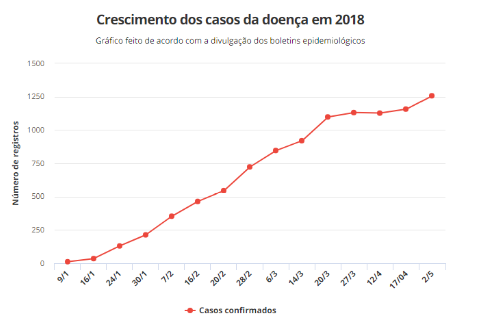
\includegraphics[width=.5\textwidth]{grafico_alteravel_epidem.png}
       
No intervalo de tempo entre julho de 2017, até a semana epidemiológica 18 de 2018, tivemos o total de 7.410 epizootias em PNH no qual 738 foram confirmados, 2.225 permanecem em investigação, 2.544 foram indeterminados e 1.903 foram descartados.

	Os maiores casos confirmados de epizootias sucederam na região Sudeste, em maior concentração na Unidade Federativa de São Paulo com 593 (80,3\% do total) eventos confirmados; já em outras regiões as notificações encontradas são em Minas Gerais 100 (13,6\% do total), Rio de Janeiro 39 (5,3 \% do total), Tocantins 3 (0,4\% dos casos) e por fim Espírito Santo com 2 casos (0,3\% do total)  e Mato Grosso 1 caso (0,1\% do total).

}% Chave que finaliza o bloco de texto com tamanho \large






\section*{Casos de Febre Amarela} % Esta linha é utilizada para colocar o título do tópico que será abordado, para alterar basta alterar o que está escrito na cor preta dentro das chaves

	{\large %%%Está linha é utilizada para aumentar a fonte pois a fonte padrão do latex é menor, não é necessário alterar essa parte,a menos que seja necessário alterar tamanho da fonte. Neste caso, \large pode ser alterado para uma dessas opções da menor para maior: \tiny, \scriptsize, \footnotesize, \small, \normalsize, \arge, \Large, \huge, \Huge .
    
   % Esta parte é utilizada para colocar o texto do tópico, para alterar basta alterar o que está escrito na cor preta dentro das chaves
    
    Até a semana epidemiológica 18 de 2018 no período de monitoramento julho de 2017/junho de 2018 foram notificados 6.525 casos suspeitos de Febre Amarela, sendo que, destes 3.963 foram descartados, 1.301 estão em investigação e 1.261 foram confirmados (Tabela 1). A maior porcentagem de casos confirmados ocorreu no estado de São Paulo com 41\% de casos. Seguindo por Minas Gerais 40,9\%, Rio de Janeiro 17,5\%, Espírito Santo 0,5\% e Distrito Federal 0,1\%.
    
	De todos os casos confirmados, 852 evoluíram para cura (67,6\% do total) e 409 para óbito, letalidade de 32,4\%.
}%%%%%% Chave que finaliza o bloco de texto com tamanho \large



\section*{Óbitos}% Esta linha é utilizada para colocar o título do tópico que será abordado, para alterar basta alterar o que está escrito na cor preta dentro das chaves

	{\large%%%Está linha é utilizada para aumentar a fonte pois a fonte padrão do latex é menor, não é necessário alterar essa parte, a menos que seja necessário alterar tamanho da fonte. Neste caso, \large pode ser alterado para uma dessas opções da menor para maior: \tiny, \scriptsize, \footnotesize, \small, \normalsize, \arge, \Large, \huge, \Huge .
    
   % Esta parte é utilizada para colocar o texto do tópico, para alterar basta alterar o que está escrito na cor preta dentro das chaves
    
	Dados atualizados disponibilizados pelo Ministério da Saúde dispõe de quantidades mais elevadas de óbitos em Minas Gerais, São Paulo e Rio de Janeiro demonstram no período entre julho de 2017 ao dia 05 de maio de 2018 (Semana Epidemiológica 18), um crescente número de óbitos confirmados.
	No estado de Minas Gerais foram confirmados 176 óbitos em decorrência de febre amarela. O estado de São Paulo demonstrou um total de 160 óbitos. No Rio de Janeiro foram confirmados 71 óbitos no mesmo período. Foi confirmado 1 óbito nos estados do Distrito Federal e Espirito Santo. (Tabela 1)

	A taxa de letalidade indica o percentual de pessoas que morreram pelo agravo e pode informar a qualidade da assistência médica a população. Sendo assim, o Distrito Federal apresentou letalidade de 100\%, Minas Gerais 34,1\% , o Rio de Janeiro 32,1\%, São Paulo 30,9\% e Santo 16,7\%. (Imagem 1)
} %%Chave que finaliza o bloco de texto com tamanho \large





\section*{Perfil demográfico}% Esta linha é utilizada para colocar o título do tópico que será abordado, para alterar basta alterar o que está escrito na cor preta dentro das chaves

	{\large %%%%Está linha é utilizada para aumentar a fonte pois a fonte padrão do latex é menor, não é necessário alterar essa parte,a menos que seja necessário alterar tamanho da fonte. Neste caso, \large pode ser alterado para uma dessas opções da menor para maior: \tiny, \scriptsize, \footnotesize, \small, \normalsize, \arge, \Large, \huge, \Huge .
    
    % Esta parte é utilizada para colocar o texto do tópico, para alterar basta alterar o que está escrito na cor preta dentro das chaves
     
	A partir da análise dos dados sobre a Febre Amarela, podemos demonstrar  que a maioria dos casos sucedem em individuos do sexo masculino, em idade economicamente ativa.
    
	Levando em consideração que as regiões mais afetadas  são as que não posssuiam recomendação de vacina anteriormente, como o Sudeste.
Sendo que São Paulo centraliza a maior parte dos óbitos (82\% do total), com base dados do Ministério da Saúde.
}%Chave que finaliza o bloco de texto com tamanho \large

	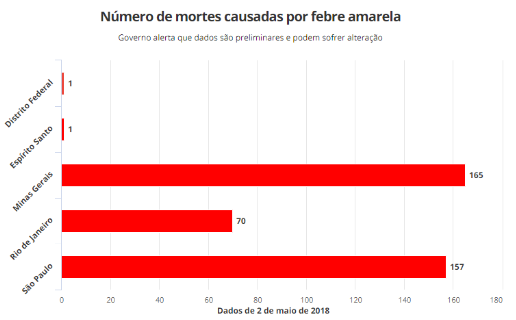
\includegraphics[width=.5\textwidth]{img_alteravel_boletim_ep.png}
{\small Fonte: Ministério da Saúde} % Este espaço serve para colocar a imagem desejada, a imagem irá aparecer justificado em harmonia com o texto colocado, para alterar a imagem basta inserir a imagem no canto superior esquerdo na aba "project", e assim irá abrir uma nova aba escrito "file", agora é necessário clicar na palavra "files" que está na cor cinza com um ícone de pasta ao lado, quando clicado no ícone "file" irá abrir uma janela com várias opções, aí é necessário selecionar a 9ª opção denominada "computer" que está no subitem uploade... computer, a escolha é de selecionar a imagem do computador e após a escolha é necessário clicar em enviar; após fazer isso é necessário observar qual o nome da imagem, e aí é necessário apenas acrescentar o nome da imagem nas chaves abaixo, conforme exemplo {capa_boletim_epidemiologico.png} é necessário colocar a extensão da imagem (no caso o .png), caso a imagem seja .jpg é necessário alterar o .png para o .jpg %




\section*{Diminuição de casos com o inverno e vacinação} % Esta linha é utilizada para colocar o título do tópico que será abordado, para alterar basta alterar o que está escrito na cor preta dentro das chaves

   {\large %%Está linha é utilizada para aumentar a fonte pois a fonte padrão do latex é menor, não é necessário alterar essa parte,a menos que seja necessário alterar tamanho da fonte. Neste caso, \large pode ser alterado para uma dessas opções da menor para maior: \tiny, \scriptsize, \footnotesize, \small, \normalsize, \arge, \Large, \huge, \Huge .
   
    % Esta parte é utilizada para colocar o texto do tópico, para alterar basta alterar o que está escrito na cor preta dentro das chaves
	É esperado que com a divulgação das vacinas o número de casos e mortes sejam diminuidos, principalmente na proximidades do inverno levando em consideração que o vírus da febre amarela tem sua circulação com mais frequencia no verão.
	
    Nesse período foi encaminhado dados que apresentam a quantidade de 25,1 milhões de dose de vacinas contra febre amarela a todos estado brasileiro. Rio de Janeiro, Bahia e São Paulo foram enviados cerca de 18,4 milhões de dose.
}%%Chave que finaliza o bloco de texto com tamanho \large

\end{multicols*}



\newpage %%esta linha é utilizada para criar uma nova página 



%Início da Tabela

\justifying
	\section*{\large{TABELA 1 - Distribuição dos casos suspeitos de Febre Amarela notificados à SVS/MS por UF de provável infecção e classificação, Brasil, monitoramento 2017/2018, SE 18, (jul/17 a jun/18).}} %Esta linha é utilizada para o título principal da tabela, para alterar o título é necessário apenas trocar a frase na cor preta pela frase desejada
 
 
 
% modelo da tabela%  %Esta parte define a formatação da tabela desejada, conforme conversado anteriormente a parte da tabela que será editado será apenas os números, pois a os nomes das regiões e os tipos de casos permanecerão sem alteração, apenas alterar os números

\begin{table}[h!] 
\justifying
\label{my-label}
\begin{tabular}{llllll} %Esta linha é utilizada para definir quantas colunas serão, para adicionar ou diminuir colunas é necessário colocar mais um l dentro das chaves, caso adicione ou diminua as colunas é necessário também alterar nos subtítulos e nas colunas.
\\\hline

\bf{\calibrifont Região/ Unidade da} & \bf{\calibrifont Casos} & \bf{\calibrifont Casos} & \bf{\calibrifont Casos} & \bf{\calibrifont Casos} \\ \bf{\calibrifont Federação} & \bf{\calibrifont Notificados} & \bf{\calibrifont Descartados} & \bf{\calibrifont em Investigação} & \bf{\calibrifont confirmados} & \bf{\calibrifont Óbitos} \\ \hline %esta linha é utilizada para colocar os subtítulos da tabela, para alterar os nomes basta trocar a frase que está na cor preta pela frase desejada


  % VALORES EDITÁVEIS (NÚMEROS) - Esta é a parte editável, é necessário observar que as edições são por linhas e não por colunas, logo para alterar os valores da coluna do Acre(por exemplo) é necessário alterar apenas a linha que está o nome do Acre. São separados por região, logo cada região tem o seu subítulo principal e logo após as suas regiões.
 \bf{\calibrifont Norte} & \bf{\calibrifont 96} & \bf{\calibrifont 69} & \bf{\calibrifont 27} & \bf{\calibrifont -} & \bf{\calibrifont -} \\ \hline
 
\calibri{Acre} & \calibri{2} & \calibri{1} & \calibri{1} & \calibri{-} & \calibri{-} \\
\calibri{Amapá} & \calibri{6} & \calibri{4} & \calibri{2} & \calibri{}  & \calibri{} \\
\calibri{Amazonas}  & \calibri{8} & \calibri{5} & \calibri{3} & \calibri{-}  & \calibri{-}  \\
\calibri{Pará}  & \calibri{46} & \calibri{33} & \calibri{13} & \calibri{-}  & \calibri{-} \\
\calibri{Rondônia}  & \calibri{9} & \calibri{8} & \calibri{1} & \calibri{-}  & \calibri{-} \\
\calibri{Roraima}  & \calibri{3} & \calibri{3} & \calibri{0} & \calibri{-}  & \calibri{-} \\
\calibri{Tocantins}  & \calibri{22} & \calibri{15} & \calibri{7} & \calibri{-}  & \calibri{-} \\

 % VALORES EDITÁVEIS (NÚMEROS) - Esta é a parte editável, é necessário observar que as edições são por linhas e não por colunas, logo para alterar os valores da coluna do Acre(por exemplo) é necessário alterar apenas a linha que está o nome do Acre. São separados por região, logo cada região tem o seu subítulo principal e logo após as suas regiões.
\hline
 \bf{\calibrifont Nordeste} & \bf{\calibrifont 123} & \bf{\calibrifont 79} & \bf{\calibrifont 44} & \bf{\calibrifont -} & \bf{\calibrifont -} \\ \hline
 
\calibri{Alagoas} & \calibri{8} & \calibri{8} & \calibri{-} & \calibri{-} & \calibri{-} \\
\calibri{Bahia} & \calibri{70} & \calibri{45} & \calibri{25} & \calibri{-} & \calibri{-} \\
\calibri{Ceará} & \calibri{4} & \calibri{3} & \calibri{1} & \calibri{-} & \calibri{-} \\
\calibri{Maranhão} & \calibri{9} & \calibri{7} & \calibri{2} & \calibri{-} & \calibri{-} \\
\calibri{Paraíba} & \calibri{5} & \calibri{0} & \calibri{5} & \calibri{} & \calibri{} \\
\calibri{Pernambuco} & \calibri{8} & \calibri{5} & \calibri{3} & \calibri{-} & \calibri{-} \\
\calibri{Piauí} & \calibri{11} & \calibri{6} & \calibri{5} & \calibri{-} & \calibri{-} \\
\calibri{Rio Grande do Norte} & \calibri{5} & \calibri{2} & \calibri{3} & \calibri{} & \calibri{} \\
\calibri{Sergipe} & \calibri{3} & \calibri{3} & \calibri{0} & \calibri{-} & \calibri{-} \\

 % VALORES EDITÁVEIS (NÚMEROS) - Esta é a parte editável, é necessário observar que as edições são por linhas e não por colunas, logo para alterar os valores da coluna do Acre(por exemplo) é necessário alterar apenas a linha que está o nome do Acre. São separados por região, logo cada região tem o seu subítulo principal e logo após as suas regiões.
\hline
 \bf{\calibrifont Sudeste} & \bf{\calibrifont 5890} & \bf{\calibrifont 3490} & \bf{\calibrifont 1140} & \bf{\calibrifont 1260} & \bf{\calibrifont 408} \\ \hline

\calibri{Espírito Santo} & \calibri{127} & \calibri{104} & \calibri{17} & \calibri{6} & \calibri{1} \\
\calibri{Minas Gerais} & \calibri{1566} & \calibri{815} & \calibri{235} & \calibri{516} & \calibri{176} \\
\calibri{Rio de Janeiro} & \calibri{1323} & \calibri{622} & \calibri{480} & \calibri{221} & \calibri{71} \\
\calibri{São Paulo} & \calibri{2874} & \calibri{1949} & \calibri{408} & \calibri{517} & \calibri{160} \\

  % VALORES EDITÁVEIS (NÚMEROS) - Esta é a parte editável, é necessário observar que as edições são por linhas e não por colunas, logo para alterar os valores da coluna do Acre(por exemplo) é necessário alterar apenas a linha que está o nome do Acre. São separados por região, logo cada região tem o seu subítulo principal e logo após as suas regiões.
\hline
 \bf{\calibrifont Sul} & \bf{\calibrifont 233} & \bf{\calibrifont 188} & \bf{\calibrifont 45} & \bf{\calibrifont -} & \bf{\calibrifont -} \\ \hline
 
\calibri{Paraná} & \calibri{126} & \calibri{119} & \calibri{7} & \calibri{-} & \calibri{-} \\
\calibri{Rio Grande do Sul} & \calibri{56} & \calibri{41} & \calibri{15} & \calibri{-} & \calibri{-} \\
\calibri{Santa Catarina} & \calibri{51} & \calibri{28} & \calibri{23} & \calibri{-} & \calibri{-} \\

 % VALORES EDITÁVEIS (NÚMEROS) - Esta é a parte editável, é necessário observar que as edições são por linhas e não por colunas, logo para alterar os valores da coluna do Acre(por exemplo) é necessário alterar apenas a linha que está o nome do Acre. São separados por região, logo cada região tem o seu subítulo principal e logo após as suas regiões.
\hline
 \bf{\calibrifont Centro-Oeste} & \bf{\calibrifont 183} & \bf{\calibrifont 137} & \bf{\calibrifont 45} & \bf{\calibrifont 1} & \bf{\calibrifont 1} \\ \hline

\calibri{Distrito Federal} & \calibri{81} & \calibri{72} & \calibri{8} & \calibri{1} & \calibri{1} \\
\calibri{Goiás} & \calibri{75} & \calibri{44} & \calibri{31} & \calibri{-} & \calibri{-} \\
\calibri{Mato Grosso} & \calibri{14} & \calibri{10} & \calibri{4} & \calibri{-} & \calibri{-} \\
\calibri{Mato Grosso do Sul} & \calibri{13} & \calibri{11} & \calibri{2} & \calibri{-} & \calibri{-} \\

 % VALORES EDITÁVEIS (NÚMEROS) - Esta é a parte editável, é necessário observar que as edições são por linhas e não por colunas, logo para alterar os valores da coluna do Acre(por exemplo) é necessário alterar apenas a linha que está o nome do Acre. Esta é a linha que define o total de todas as regiões do Brasil
\hline
 \bf{\calibrifont Brasil} & \bf{\calibrifont 6525} & \bf{\calibrifont 3963} & \bf{\calibrifont 1301} & \bf{\calibrifont 1261} & 

\bf{\calibrifont 409} \\ \hline
\end{tabular}
\end{table}
 	 {\timesfont \textbf{Fonte}: Sinan; CGDT/DEVIT/SVS/MS.}

%Fim da Tabela
     
     
     
     
\newpage
	\section*{\large{Imagem 1 - Taxa de letalidade por Febre Amarela, por Unidade da Federação, Brasil, julho 2017/ 05 maio 2018.}} %Esta linha é utilizada para definir o título da imagem final do boletim, para alterar o título basta apenas alterar a frase na cor preta pela frase desejada
    \centering
    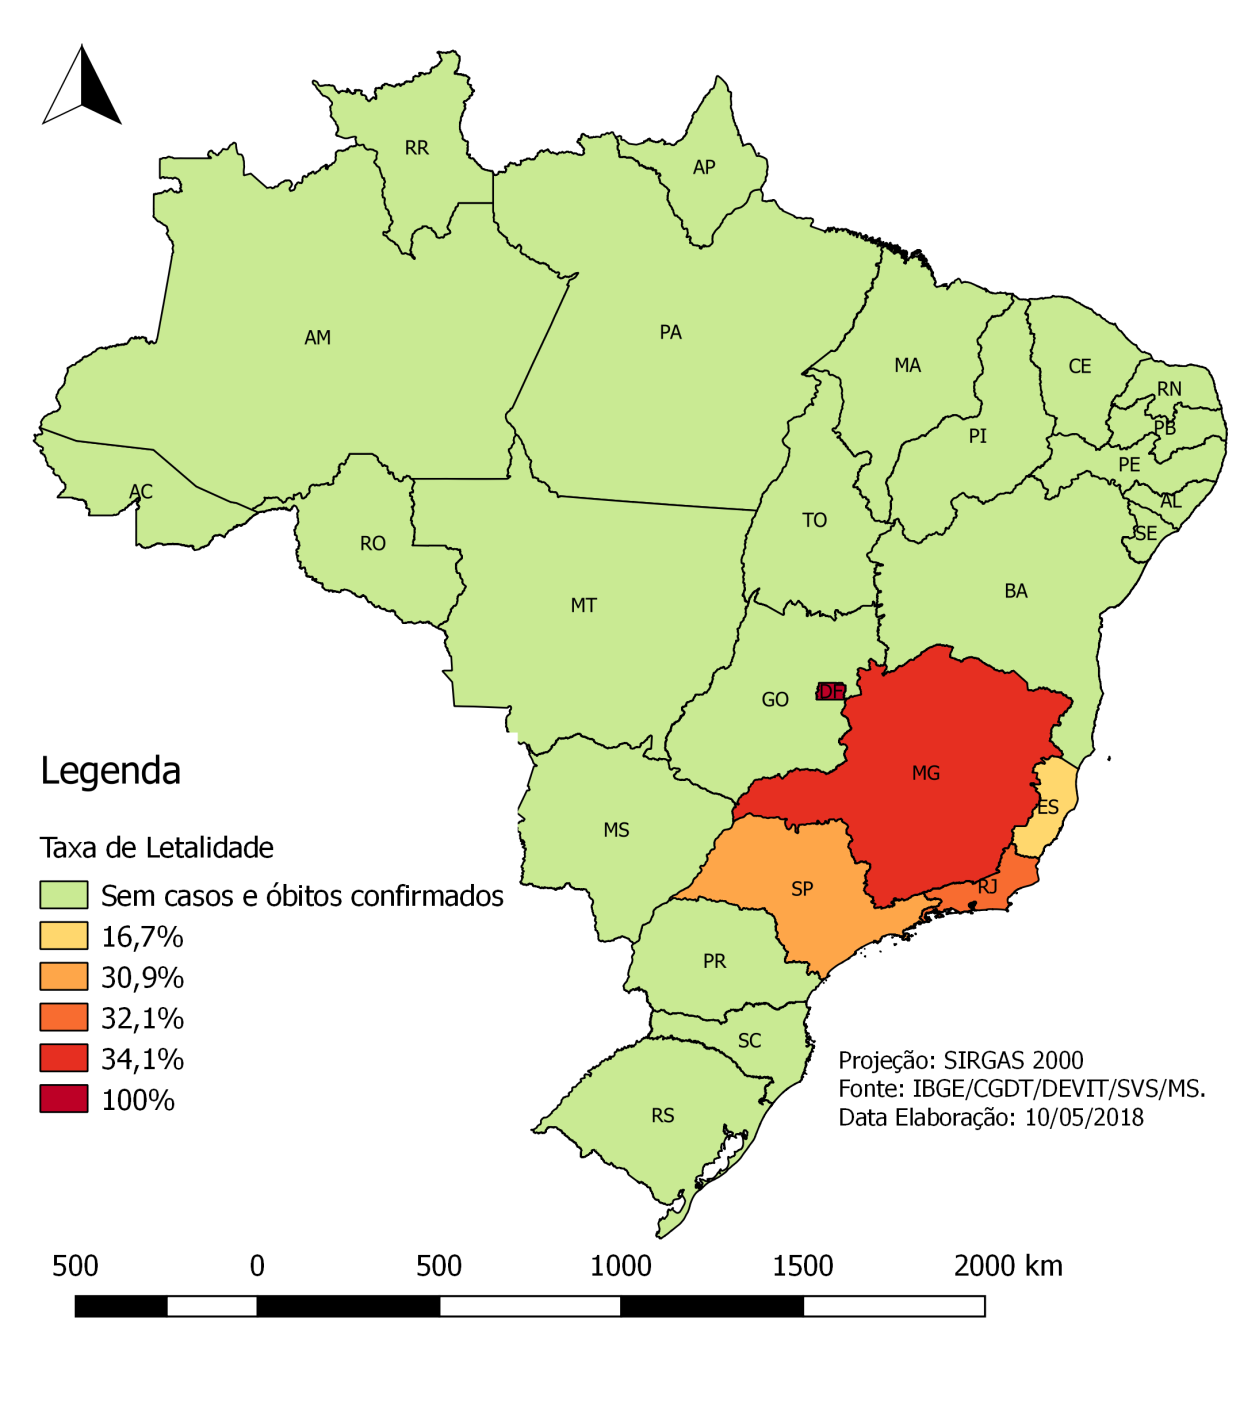
\includegraphics[width=.8\textwidth]{mapa_alteravel_boletim_epidemi.png} % Este espaço serve para colocar a imagem desejada, a imagem irá aparecer justificado em harmonia com o texto colocado, para alterar a imagem basta inserir a imagem no canto superior esquerdo na aba "project", e assim irá abrir uma nova aba escrito "file", agora é necessário clicar na palavra "files" que está na cor cinza com um ícone de pasta ao lado, quando clicado no ícone "file" irá abrir uma janela com várias opções, aí é necessário selecionar a 9ª opção denominada "computer" que está no subitem uploade... computer, a escolha é de selecionar a imagem do computador e após a escolha é necessário clicar em enviar; após fazer isso é necessário observar qual o nome da imagem, e aí é necessário apenas acrescentar o nome da imagem nas chaves abaixo, conforme exemplo {capa_boletim_epidemiologico.png} é necessário colocar a extensão da imagem (no caso o .png), caso a imagem seja .jpg é necessário alterar o .png para o .jpg %
    
    
\newpage %Linha para criação de uma nova página


% referencias do modelo%
\section*{\centering\large{\calibrifont Referências}} %Esta linha é utilizada para o título da nova página, para alterar o título basta apenas alterar a frase na cor preta pela frase desejada

\justifying
 % Esta parte é utilizada para colocar as referências
 
	BRASIL. Monitoramento do Período Sazonal de Febre Amarela Brasil 2017/2018. Brasil: Ministério da Saúde, Secretaria de Vigilância em Saúde. N°25, 2018. Disponível em: <\url{http://portalarquivos2.saude.gov.br/images/pdf/2018/maio/09/Informe-FA.pdf}> Acesso em: 10/05/2018.
\\ \\
	 G1.  Febre amarela: Brasil regisyta 394 mortes e 1257 casos nos últimos dez meses. Disponível em: <\url{https://g1.globo.com/bemestar/noticia/brasil-registra-394-mortes-e-1257-casos-de-febre-amarela-diz-ministerio-da-saude.ghtml}>. Acesso em: 10/05/2018.
\\ \\
	COMUNICAÇÃO ICMBio. O papel dos macacos no ciclo da febre amarela.  Disponível em: <\url{http://www.olimpiada.fiocruz.br/o-papel-dos-macacos-no-ciclo-da-febre-amarela}>. Acesso em 12/04/2018
\\ \\
	MINISTÉRIO DA SAÚDE. Vacina de febre amarela será ampliada para todo o Brasil. Disponível em: <\url{http://portalms.saude.gov.br/noticias/agencia-saude/42849-vacina-de-febre-amarela-sera-ampliada-para-todo-o-brasil}> Acesso em: 12/04/2018.
\\ \\
	O GLOBO. Vírus da febre amarela é detectado em outra espécie de mosquito em MG. Disponível em: <\url{https://oglobo.globo.com/sociedade/saude/virus-da-febre-amarela-detectado-em-outra-especie-de-mosquito-em-mg-22402258}> Acesso em: 12/04/2018.


%Esta parte é a parte que das referências no rodapé da página, para alterar basta alterar as frases da cor preta para as frases desejadas
\vfill % adiciona as referencias no rodape da pagina%
\centering{

\includegraphics{logo.png} \\

  \normalsize{\bf{\calibrifont Elaboração}}\\ %  As barras: " \\ " são utilizadas para a troca de linha
  	\calibri{Maria Verônica Galeno Dias, Marina Pissurno do Nascimento, Beatriz Amaral\\
 	Ferreira da Silva}\\ %EDITÁVEL
    
	\normalsize{\bf{\calibrifont Equipe Editorial}}\\
	\calibri{Joaquim Bastos\\ %EDITÁVEL
    Sala de Situação - Faculdade de Ciências da Saúde (UnB)}\\
    
	\normalsize{\bf{\calibrifont Revisão}}\\
 	\calibri{Patrícia Paiva Pereira, Marcela Lopes Santos}\\ %EDITÁVEL
  
	\normalsize{\bf{\calibrifont Coordenação}}\\
  	\calibri{Janaina Sallas, Jonas Brant}\\ %EDITÁVEL
 	\normalsize{\bf{\calibrifont Contato}}\\
	\calibri{sdscenteias@unb.br}\\ %EDITÁVEL
}

\end{document}
